% !TeX spellcheck = ru_RU
% !TEX root = gpu_lodygin.tex

\section{Эксперимент}
В данном эксперименте проводится исследование производительности реализованной библиотеки по обработке изображений на CPU и GPU. Основная задача --- выяснить, на каком из процессоров (центральном или графическом) с использованием оптимального количества агентов будет быстрее обработан массив изображений с заданными трансформациями. В качестве оптимального количества агентов рассматривается количество логических процессоров системы.

\subsection{Условия эксперимента}
Для экспериментов использовалась рабочая станция с процессором Intel Core i5-10300H с тактовой частотой 2.50GHz, RAM DDR4 объемом 8гб, видекартой NVIDIA GeForce GTX 1650 Ti с объемом памяти 4гб под управлением OC Windows 10.

\subsection{Исследовательские вопросы }

\begin{itemize}
\item Какой из методов по обработке массива изображений быстрее, параллельная версия на CPU с использованием количества потоков, равных количеству логических процессоров или версия обработки на GPU.
\end{itemize}

\subsection{Метрики}
В качестве метрик производительности используется время, требуемое на завершение обработки. Показатели времени получены с помощью библиотеки \texttt{BenchmarkDotNet v0.13.5}\footnote{Репозиторий библиотеки \texttt{BenchmarkDotNet}: \url{https://github.com/dotnet/BenchmarkDotNet} (дата доступа:   \DTMdate{2023-05-25}).}. Для замеров были выбраны стандартные настройки по \enquote{прогреву} и количеству итераций для измерений.

\subsection{Результаты}

Замеры производились на массиве из 30 изображений с котами. Каждое изображение было повернуто два раза на $90^{\circ}$ по часовой стрелке, затем отражено по горизонтали и, наконец, к каждому изображению был применён фильтр \texttt{FishEye}. Полученные результаты приведены в таблице~\ref{processing}.

\begin{table}[h]
\centering
    \caption{Производительность обработки массива изображений с помощью CPU и GPU на 8 агентах.}
    \rowcolors{2}{black!2}{black!10}
    \begin{tabular}{| r | r |}
    \hline
        \textsc{Method} & \textsc{Time(s) $\pm$ Error} \\ 
        \hline
        CpuProcessing & $7.83 \pm 0.08$ \\ 
        GpuProcessing & $3.86 \pm 0.06$ \\
    \hline    
    \end{tabular}%
    \label{processing}
\end{table}

Данные замеры показали, что при распараллеливании задачи по обработке массива на оптимальное количество потоков для CPU, время обработки массива изображений на центральном процессоре будет превышать время обработки того же массива на графическом процессоре в два раза.

Результаты, полученные с помощью \texttt{BenchmarkDotNet} были проверены на адекватность с помощью библиотек \texttt{SciPy v1.10.1}\footnote{Сайт библиотеки \texttt{SciPy}: \url{https://scipy.org/} (дата доступа:   \DTMdate{2023-05-25}).}, \texttt{NumPy v1.24.3}\footnote{Сайт библиотеки \texttt{NumPy}: \url{https://numpy.org/} (дата доступа:\DTMdate{2023-05-25}).} и \texttt{Matplotlib v3.7.1}\footnote{Сайт библиотеки \texttt{MatPlotLib}: \url{https://matplotlib.org/} (дата доступа:   \DTMdate{2023-05-25}).} на языке \texttt{Python}. Выборку можно принять за нормальное распределение, так как был успешно пройден тест Шапиро-Уилка, а так же зачтён критерий согласия Пирсона. В случае замеров обработки на CPU pvalue равняется 0.64 и 0.72. В случае GPU --- 0.71 и 0.57. Соответствующие им гистограммы приведены на рисунке~\ref{fig:cpu} и рисунке~\ref{fig:gpu}.

\begin{figure}[H]
    \centering
    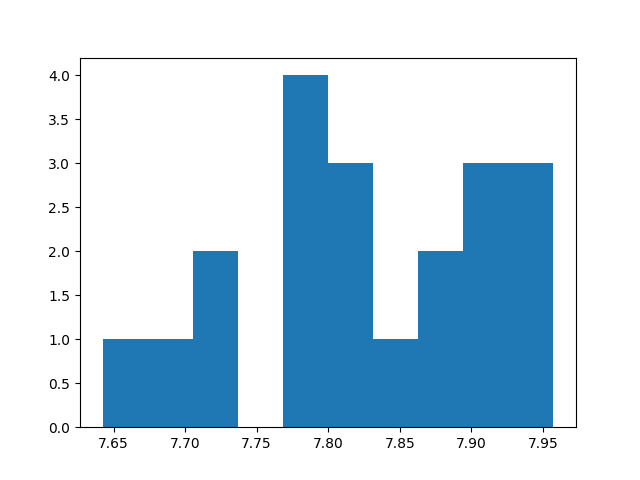
\includegraphics[width=\textwidth]{figures/CPU.png}
    \caption{Гистограмма распределения времени по обработке массива изображений на CPU}
    \label{fig:cpu}
\end{figure}

\begin{figure}[H]
    \centering
    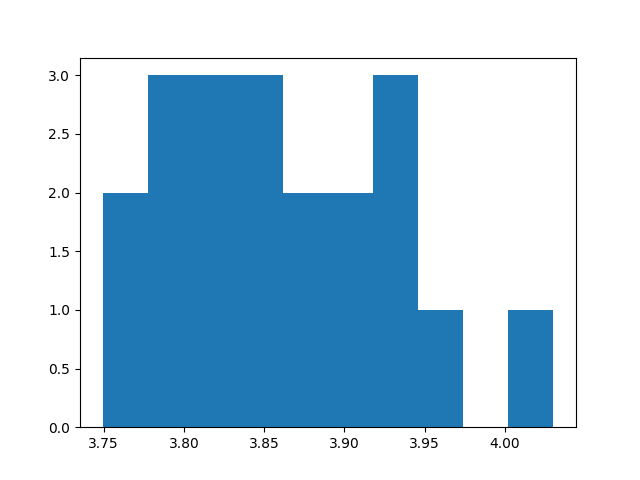
\includegraphics[width=\textwidth]{figures/GPU.png}
    \caption{Гистограмма распределения времени по обработке массива изображений на GPU}
    \label{fig:gpu}
\end{figure}

Обработанные версии на GPU и CPU идентичны. Для примера, оригинальное изображение~\ref{fig:original}, обработанное на CPU~\ref{fig:cpucat}, обработанное на GPU~\ref{fig:gpucat}.

\begin{figure}[H]
    \centering
    
\includegraphics[width=\textwidth]{figures/originalCat.jpg}
    \caption{Оригинальное изображение}
    \label{fig:original}
\end{figure}

\begin{figure}[H]
    \centering
    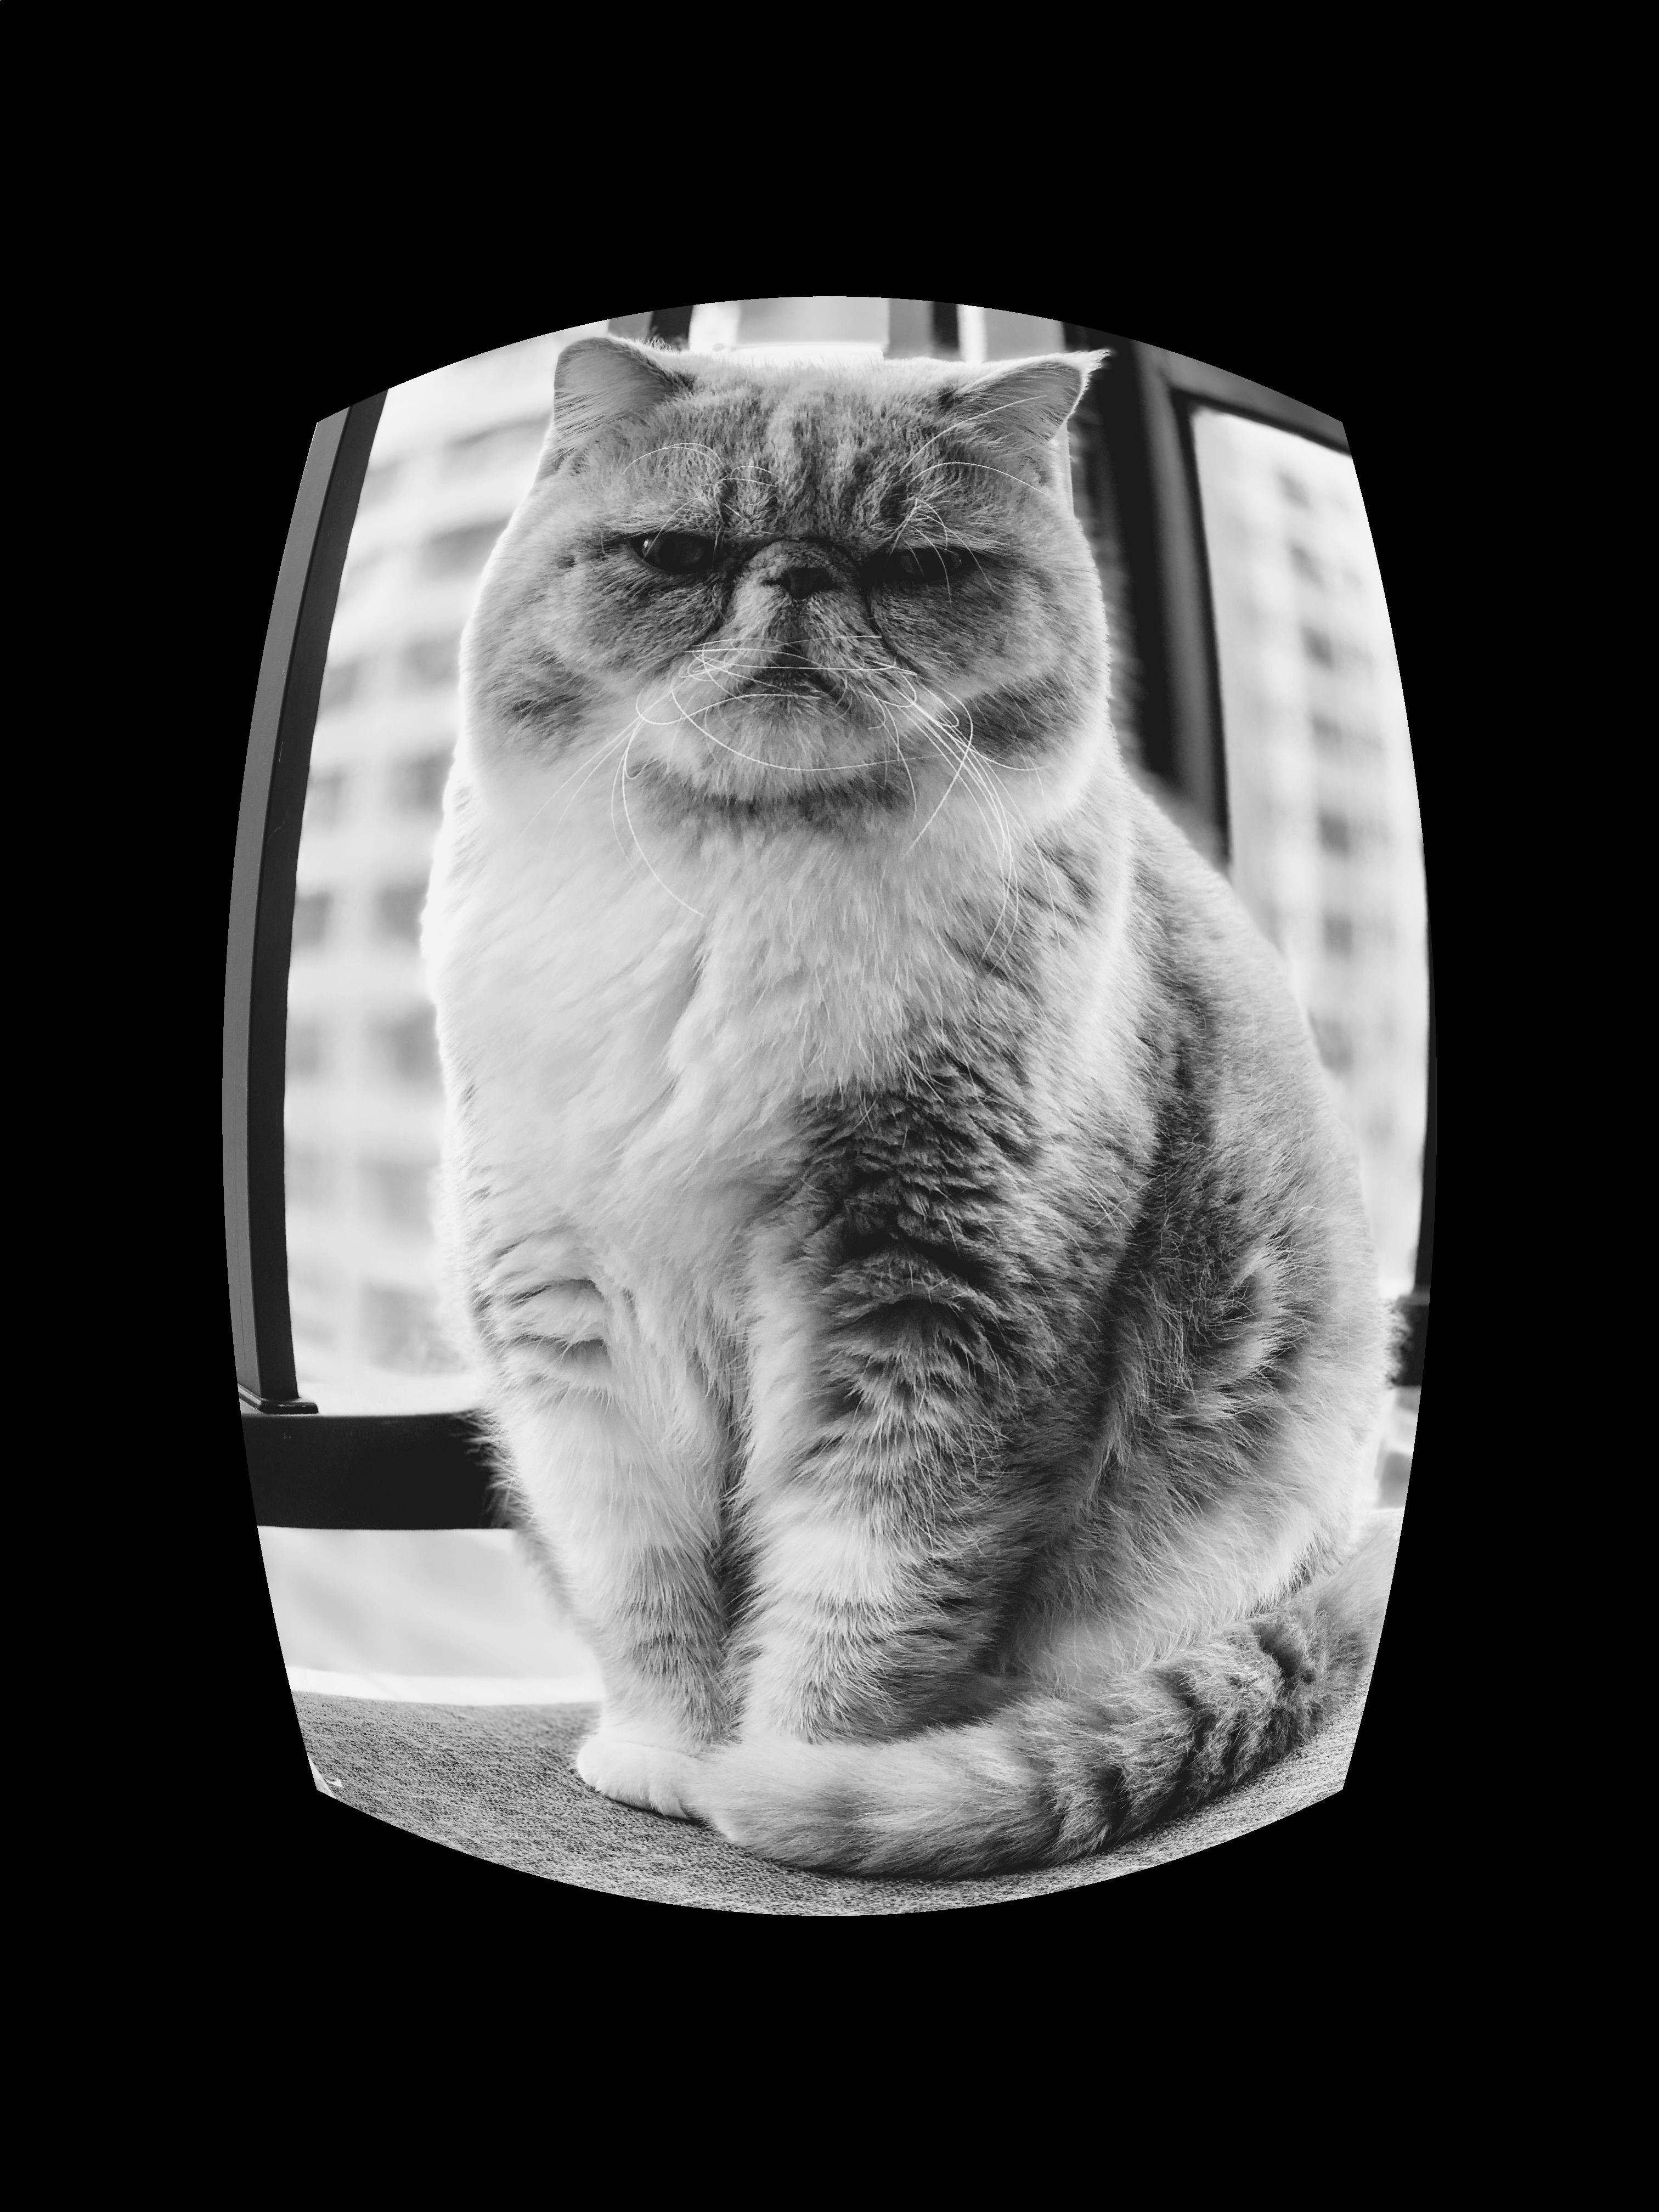
\includegraphics[width=\textwidth]{figures/CPUCat.jpg}
    \caption{Изображение после обработки на CPU}
    \label{fig:cpucat}
\end{figure}

\begin{figure}[H]
    \centering
    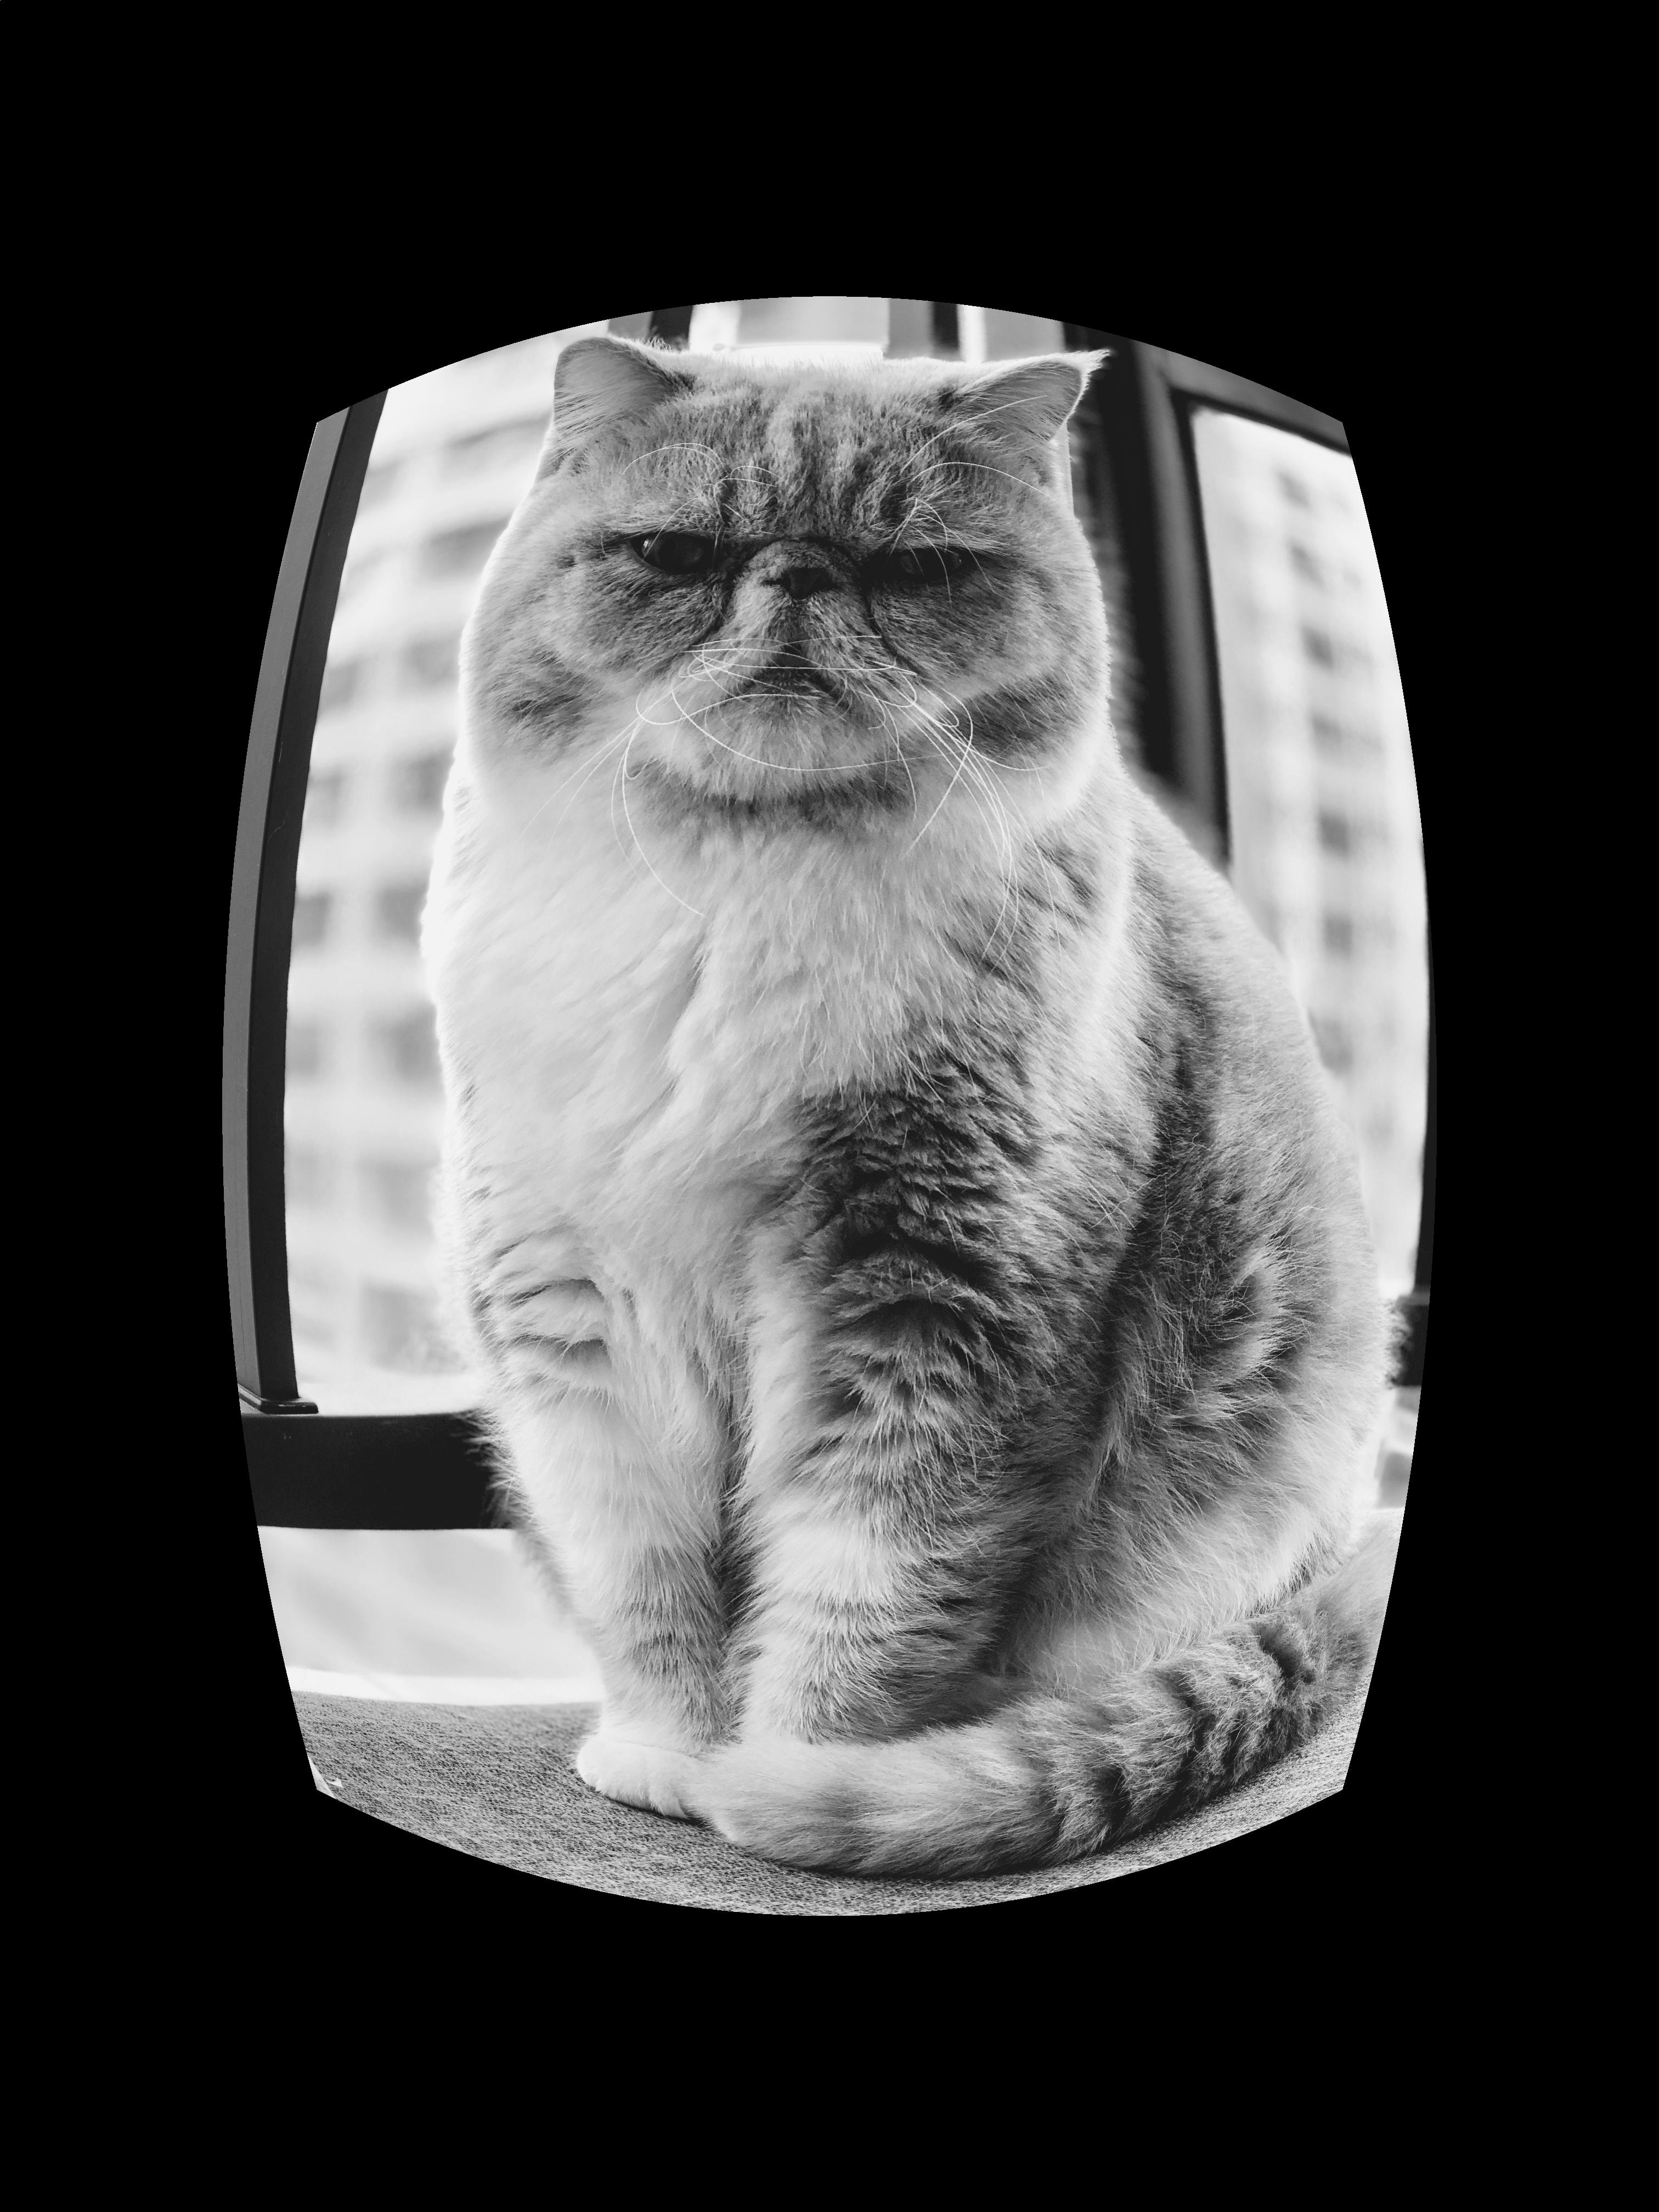
\includegraphics[width=\textwidth]{figures/GPUCat.jpg}
    \caption{Изображение после обработки на GPU}
    \label{fig:gpucat}
\end{figure}

\subsubsection{RQ1}
Исходя из полученных данных можно сделать вывод, что обработка массива изображений на GPU в два раза опережает параллельную обработку массива изображений на CPU при использовании количества потоков, равное количеству логических процессоров системы. Такой результат можно объяснить тем, что в графических процессорах используется программная модель SIMT (Single instruction, multiple threads), что позволяет выполнять одну и ту же инструкцию на гораздо большем числе независимых вычислителей.
